\chapter{Introduction to Radio Astronomy}

\section{Introduction}
Radio astronomy involves the study of radio waves from the depths of space. Many objects in the universe emit radio waves through naturally occurring processes. Such objects include stars, galaxies, and nebulae, as well as a wide variety of peculiar, fascinating, and often mysterious objects, such as pulsars and quasars. Radio astronomers study such objects using a variety of radio telescopes. Many of the astronomical objects that emit radio waves do not emit much or any light so that radio astronomers study what is essentially an invisible universe not seen by even the world’s largest optical telescopes. \\

The development of radio astronomy in the mid-twentieth century opened a new window on the universe. Before this development, astronomical observations were confined to the narrow range of visible wavelengths, limiting the range of astronomical phenomena that could be studied. The sky at radio wavelengths is vastly different from the sky observed in visible light. Stars, which are the primary sources of visible light, do not dominate the emission in the radio sky. \\

At radio wavelengths, we can detect thermal continuum and spectral-line emission from objects too cold to emit visible light. This enables the study of the cold interstellar medium of our Galaxy and others, as well as the cosmic microwave background, the relic radiation from the early universe. Nonthermal radiation, such as synchrotron emission, produces significant radio emission and is observed in a variety of astronomical sources like supernova remnants and quasars. For instance, two of the brightest sources in the radio sky, Cassiopeia A and Cygnus A, are synchrotron-emitting sources that are relatively faint at visible wavelengths. Thus, radio observations complement optical observations. \\

\clearpage

\section{Historical Development and Milestones}
The field of radio astronomy began in the early 20th century, revolutionizing our understanding of the universe by exploring it beyond visible wavelengths. The foundation for radio astronomy was laid in the 19th century through advances in electricity and magnetism, particularly with Maxwell's equations, which revealed the vast spectrum of electromagnetic radiation.

\subsection{Early Efforts and Discoveries}
In 1887, Heinrich Hertz successfully produced radio waves in a laboratory, sparking interest in detecting cosmic radio waves. Pioneering efforts in the 1890s by Thomas Edison, Arthur Kennelly, and Sir Oliver Lodge to find correlations between sunspots and radio signals failed due to the insensitivity of the equipment used. Other astronomers like Johannes Wilsing, Julius Scheiner, and Charles Nordmann also faced similar setbacks.

\subsection{Breakthroughs in the 1930s}

The critical advancement came in 1932 when Karl Jansky of Bell Labs successfully detected astronomical radio emissions while studying static interference in short-wave radio communications. Using a steerable antenna, Jansky identified a steady hiss with a directional dependence, tracing it to the plane of the Milky Way and pinpointing the galactic center as a primary source. His work, however, initially received little attention.

Intrigued by Jansky's findings, Grote Reber, an engineer, constructed a 30-foot parabolic antenna in his backyard in 1937. After initial failures at higher frequencies, Reber succeeded in mapping the galaxy's radio emissions at 160 MHz. His detailed maps identified significant sources, including the strong emission from the galactic center and secondary peaks in Cassiopeia (Cas A) and Cygnus (Cyg A). Reber's work, published in 1940 and 1944, marked the first radio wavelength observations in an astronomical journal.

\subsection{Advancements During and After World War II}

World War II brought significant technological advancements in radar, leading to critical developments in radio astronomy. In 1942, J.S. Hey of the British Army Operational Research Group linked radar jamming to sunspot activity, a hypothesis later supported by Southworth of Bell Labs, who detected radio emissions from the quiescent Sun.

Post-war, Hey and colleagues continued their radio studies, discovering in 1945 that meteor trails reflect radio waves and mapping the radio sky in greater detail than Reber. They identified Cygnus A as a discrete source and in 1948 linked solar radio bursts to sunspots and solar flares.

\subsection{The Hydrogen Line and Interferometry}

In 1944, Dutch astrophysicist Jan Oort suggested to Hendrik van de Hulst the calculation of the hydrogen emission line due to electron spin-flip transitions. Van de Hulst predicted radiation at a 21-cm wavelength, first detected by Harold Ewen and Edward Purcell at Harvard in 1951. This discovery enabled detailed hydrogen mapping in the Milky Way and remains a vital tool in radio astronomy.

In 1946, Martin Ryle and D.D. Vonberg conducted the first interferometric observations using paired radio antennas. Subsequent interferometry by various researchers provided precise positions for bright radio sources, facilitating optical identifications of objects like Cygnus A, Cassiopeia A, and the Crab Nebula. By 1959, the Third Cambridge Catalog (3C) cataloged the brightest 471 radio sources, later revised as 3CR.

\subsection{Theoretical Insights and Nobel Prizes}

The 1950s saw the understanding of synchrotron radiation, a process where relativistic electrons emit photons while spiraling around magnetic field lines, proposed by Hannes Alfvén, Nicolai Herlofsen, and Iosif Shklovsky. The 1960s brought significant discoveries, including quasars, pulsars, and the cosmic microwave background (CMB). These discoveries led to several Nobel Prizes: the 1974 prize to Anthony Hewish for the discovery of pulsars and the 1978 prize to Arno Penzias and Robert Wilson for the CMB. Further studies on pulsars and the CMB earned additional Nobel Prizes in 1993 (Joseph Taylor and Russell Hulse) and 2006 (John Mather and George Smoot).

\clearpage

\section{Fundamentals of Radio Waves}

This section provides a basic introduction to radio waves and electromagnetic radiation, essential for understanding radio astronomy.

\subsection{Electromagnetic Radiation}

Radio waves are a form of electromagnetic (EM) radiation, similar to visible light but at much lower frequencies. EM radiation consists of oscillating electric and magnetic fields that are perpendicular to each other and to the direction of propagation (Figure~\ref{fig:em_waves}).

\begin{figure}[H]
    \centering
    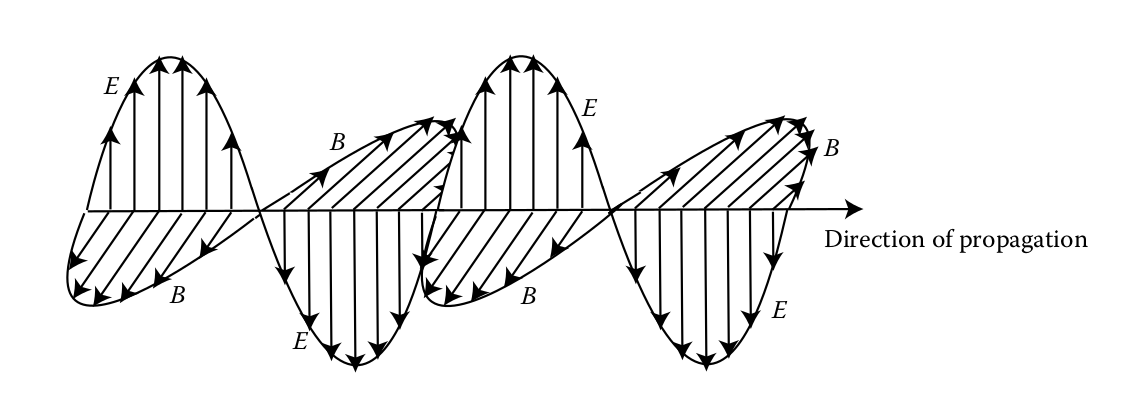
\includegraphics[width=0.7\textwidth]{Images/em_waves.png}
    \caption{Waves of electromagnetic radiation.}
    \label{fig:em_waves}
\end{figure}

The speed of EM waves in a vacuum is the speed of light, $c = 299 792 458$ m/s. The frequency, $\nu$, in hertz (Hz), and the wavelength, $\lambda$, in meters, are related by

\begin{equation}
    \lambda \nu = c
\end{equation}

EM waves are often generated by accelerating charged particles, typically electrons due to their smaller mass compared to protons. Light can be described both as a wave and as a particle (photon). The energy of a photon is given by

\begin{equation}
    E = h\nu = \frac{hc}{\lambda}
\end{equation}

where $h$ is Planck’s constant, $h = 6.626 \times 10^{-34}$ J s. The electromagnetic spectrum covers a wide range of frequencies and wavelengths (Figure~\ref{fig:em_spectrum}).

\begin{figure}[H]
    \centering
    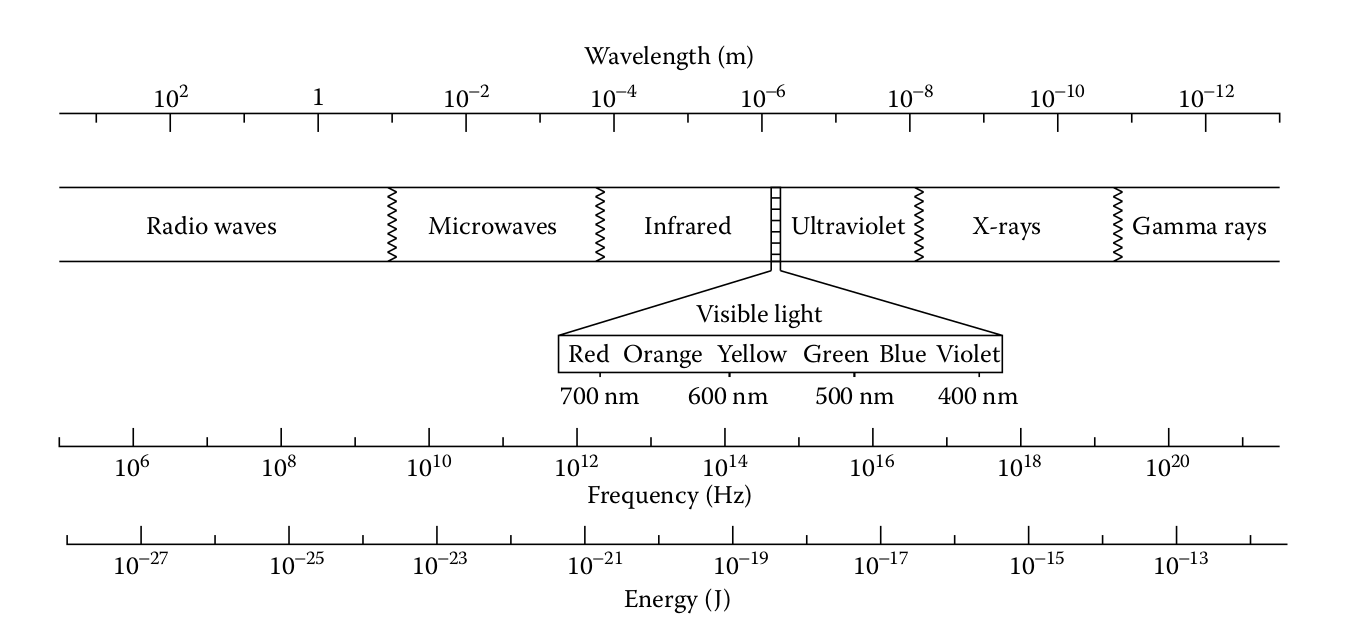
\includegraphics[width=0.7\textwidth]{Images/em_spectrum.png}
    \caption{The electromagnetic spectrum.}
    \label{fig:em_spectrum}
\end{figure}

The radio band spans from 10 MHz to 300 GHz (30 m to 1 mm in wavelength). The Earth's atmosphere allows radio waves within this range to reach the surface, except at very low frequencies (below 10 MHz) and high frequencies (above 300 GHz) due to ionospheric and atmospheric absorption.

\subsection{Spectroscopy}

Spectroscopy involves analyzing the spectrum (intensity vs. frequency or wavelength) of detected radiation, providing valuable information about the source. Classical spectrographs use prisms or gratings to separate wavelengths (Figure~\ref{fig:spectrograph}).

\begin{figure}[H]
    \centering
    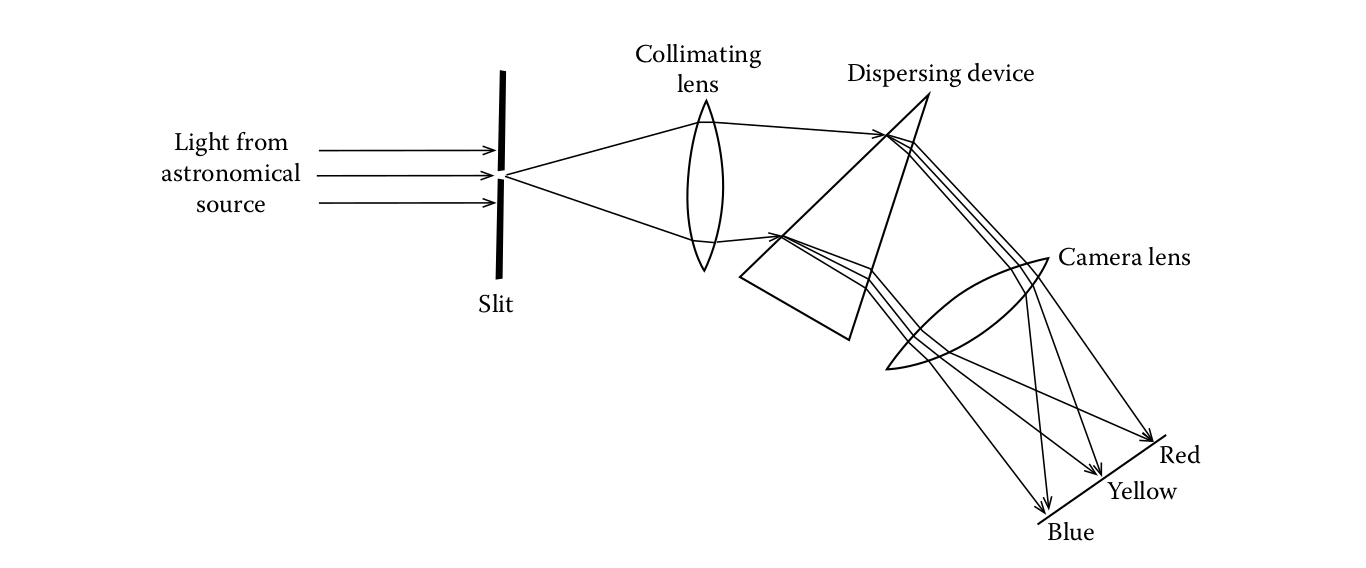
\includegraphics[width=0.7\textwidth]{Images/spectrograph.png}
    \caption{A classical spectrograph setup.}
    \label{fig:spectrograph}
\end{figure}

Radio spectrographs separate frequencies electronically, displaying the spectrum as intensity vs. frequency. There are three types of spectra based on Kirchhoff’s rules:

\begin{enumerate}
    \item \textbf{Continuous spectra:} Emission at all frequencies without breaks. An example is an incandescent lamp (Figure~\ref{fig:continuous_spectrum}).

    \begin{figure}[H]
        \centering
        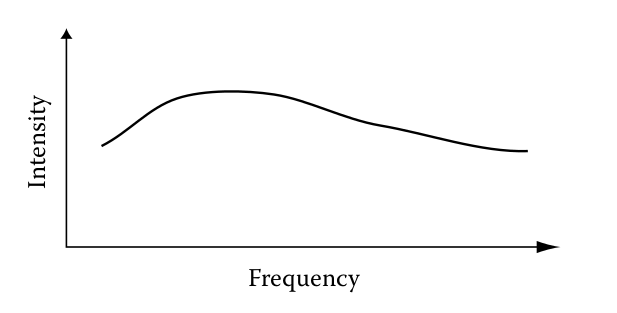
\includegraphics[width=0.7\textwidth]{Images/continuous_spectrum.png}
        \caption{Qualitative example of a continuous spectrum.}
        \label{fig:continuous_spectrum}
    \end{figure}

    \item \textbf{Emission line spectra:} Emission at specific frequencies due to quantum transitions in atoms or molecules (Figure~\ref{fig:emission_spectrum}).

    \begin{figure}[H]
        \centering
        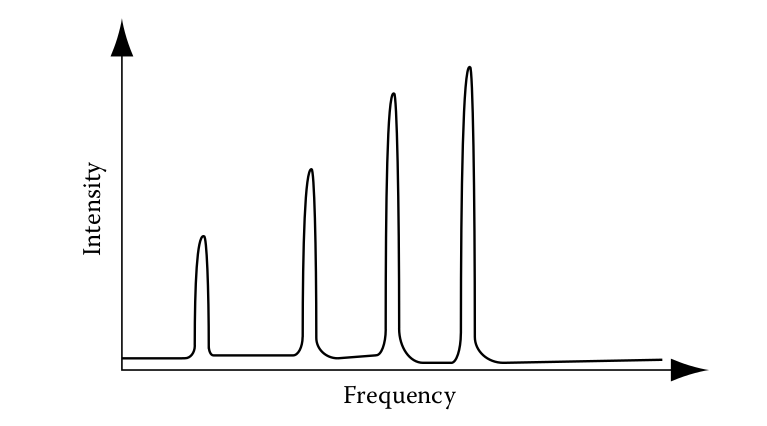
\includegraphics[width=0.7\textwidth]{Images/emission_spectrum.png}
        \caption{Qualitative sketch of an emission line spectrum.}
        \label{fig:emission_spectrum}
    \end{figure}

    \item \textbf{Absorption line spectra:} Dark lines appear when radiation passes through a cooler gas, which absorbs specific frequencies (Figure~\ref{fig:absorption_spectrum}).

    \begin{figure}[H]
        \centering
        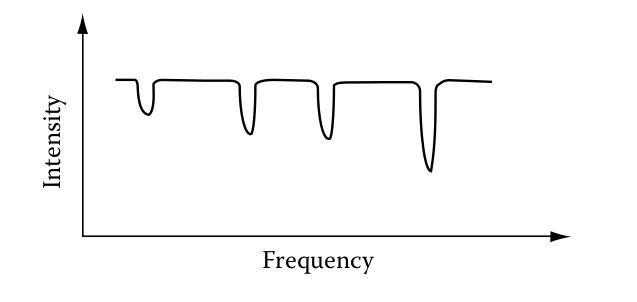
\includegraphics[width=0.7\textwidth]{Images/absorption_spectrum.png}
        \caption{Qualitative example of an absorption line spectrum.}
        \label{fig:absorption_spectrum}
    \end{figure}
\end{enumerate}

The specific frequencies of emission and absorption lines allow identification of the chemical composition of the source or intervening gas.

\clearpage

\section{Sky Coodinate System}

\subsection{Right Ascension and Declination}
To locate objects in the sky, we use a coordinate system similar to Earth's. The celestial sphere, an imaginary globe surrounding Earth, uses extensions of longitude (right ascension, RA, $\alpha$) and latitude (declination, Dec, $\delta$) lines. The celestial poles align with Earth's poles, and the sky appears to rotate about an axis through these poles.

\begin{figure}[H]
    \centering
    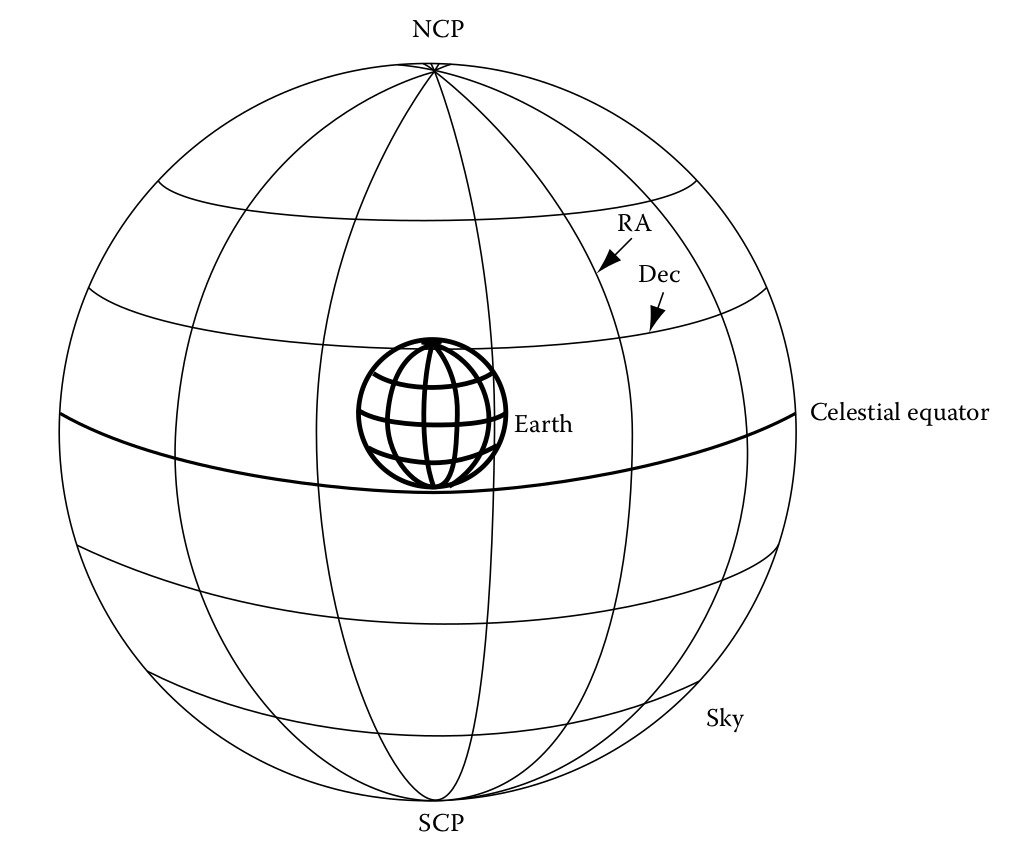
\includegraphics[width=0.7\textwidth]{Images/ra_dec.png}
    \caption{The celestial sphere with RA and Dec lines.}
    \label{fig:ra_dec}
\end{figure}

Declination is analogous to latitude and is measured in degrees from the celestial equator. RA, fixed relative to the stars, is defined such that the $0^\circ$ line of RA aligns with the $0^\circ$ line of longitude at noon on the first day of spring. RA is measured in hours, minutes, and seconds, with $24\,h$ of RA corresponding to $360^\circ$.

The units of RA are time-based due to historical reasons and simplify calculations involving Earth's rotation. The conversion between RA and degrees at the equator is $1\,h$ RA = $15^\circ$ arc, $1\, \min$ RA = $15\, \min$ arc, and $1\,s$ RA = $15\,s$ arc. Away from the equator, the angular separation between RA lines depends on declination ($\delta$) and is given by:
\[
\text{Seconds of arc} = 15 \cos (\delta) \times \text{seconds of RA}
\]

On sky maps, east appears to the left, and RA increases to the left, due to the observer's perspective relative to the ground.

\subsection{Observer-Centered Definitions}
\begin{enumerate}
    \item \textbf{Horizon}: The boundary of visible sky, blocked by the ground.
    \item \textbf{Zenith}: The point directly overhead.
    \item \textbf{Altitude/Elevation}: Angular height above the horizon ($0^\circ$ at horizon, $90^\circ$ at zenith).
    \item \textbf{Azimuth}: Angular position along the horizon from north ($0^\circ$ north, $180^\circ$ south, $90^\circ$ east, $270^\circ$ west).
    \begin{figure}[H]
        \centering
        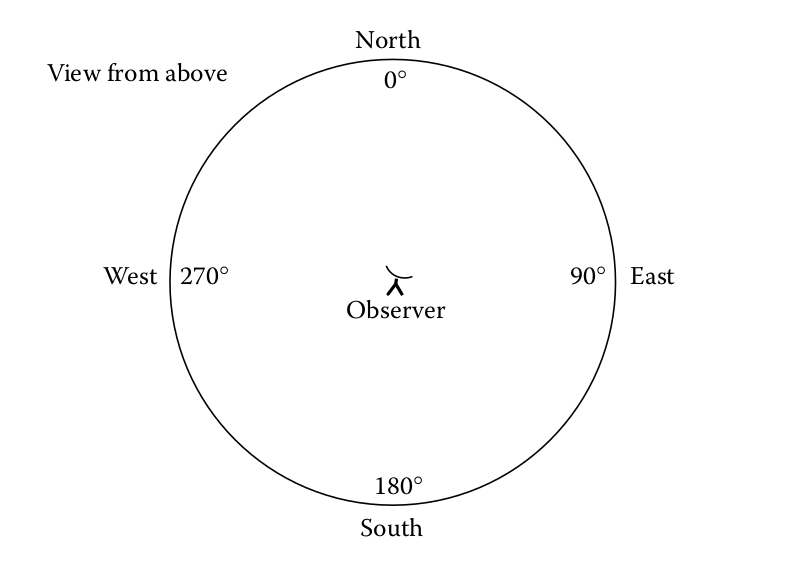
\includegraphics[width=0.7\textwidth]{Images/azimuthal_angles.png}
        \caption{View from above depicting azimuthal angles along with the cardinal directions around the horizon.}
        \label{fig:azimuthal_angles}
    \end{figure}
    \item \textbf{Meridian}: The line of RA through your zenith, connecting to celestial poles.
    \begin{figure}[H]
        \centering
        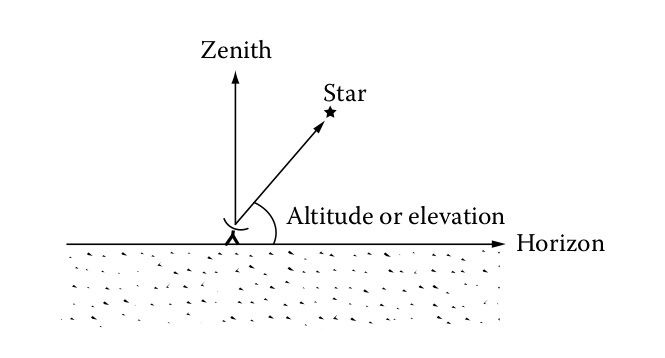
\includegraphics[width=0.7\textwidth]{Images/zenith_horizon_altitude_elevation.png}
        \caption{Schematic diagram showing the relations between zenith, horizon, and altitude or elevation.}
        \label{fig:zenith_horizon_altitude_elevation}
    \end{figure}
    \item \textbf{Transit}: When an object crosses your meridian, highest in the sky.
    \item \textbf{Hour Angle (HA)}: Hours since an object crossed your meridian.
    \item \textbf{Local Sidereal Time (LST)}: RA currently on your meridian, running slightly faster than solar time. (HA = LST - RA)
    \item \textbf{Universal Time (UT)}: Local solar time at Greenwich, England, standardized for timekeeping.
\end{enumerate}

RA measured in time simplifies finding when objects cross the meridian and explains its increase to the east.

\begin{figure}[H]
    \centering
    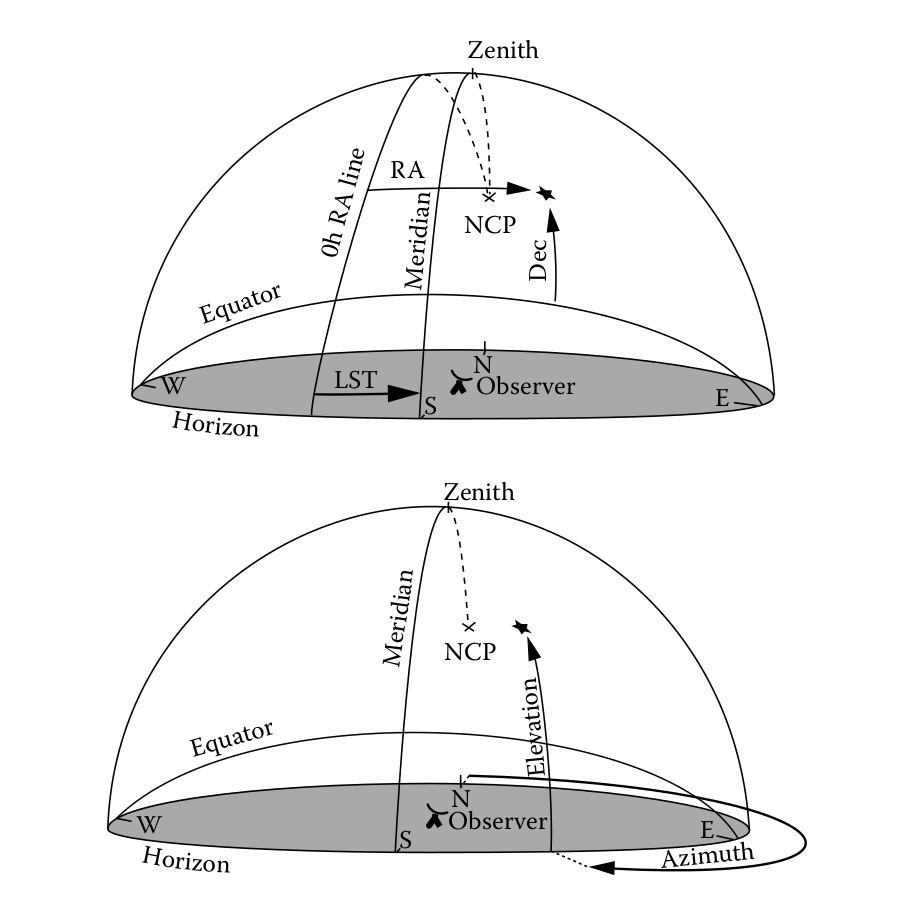
\includegraphics[width=0.7\textwidth]{Images/sky_coordinates_example.png}
    \caption{Example of sky coordinates as viewed by the observer (top) and observer-centered coordinates (bottom).}
    \label{fig:sky_coordinates_example}
\end{figure}

\subsection{Apparent Sizes}
Angular size, dependent on an object's actual size and distance, is measured in radians:
\[
\theta \, (\text{radians}) = \frac{s}{r}
\]
For small angles:
\[
\theta \, (\text{radians}) \approx \frac{l}{d}
\]
In two dimensions, the solid angle $\Omega$ is:
\[
\Omega = \frac{A}{d^2}
\]
with the unit steradian (sr), and the whole sky covering $4\pi$ sr.

Understanding these coordinate systems allows us to locate and observe celestial objects from any Earth location and describe their apparent positions and sizes accurately.


\clearpage

\section{Radio Telescopes}

Observing with a radio telescope differs significantly from using a visible-wavelength telescope. The Sun does not illuminate the entire sky at radio wavelengths, resulting in a dark daytime sky suitable for observations day and night. Long radio wavelengths penetrate clouds, whereas shorter wavelengths require clear skies due to water-induced signal loss.

A traditional radio telescope comprises five basic parts.

\begin{figure}[H]
    \centering
    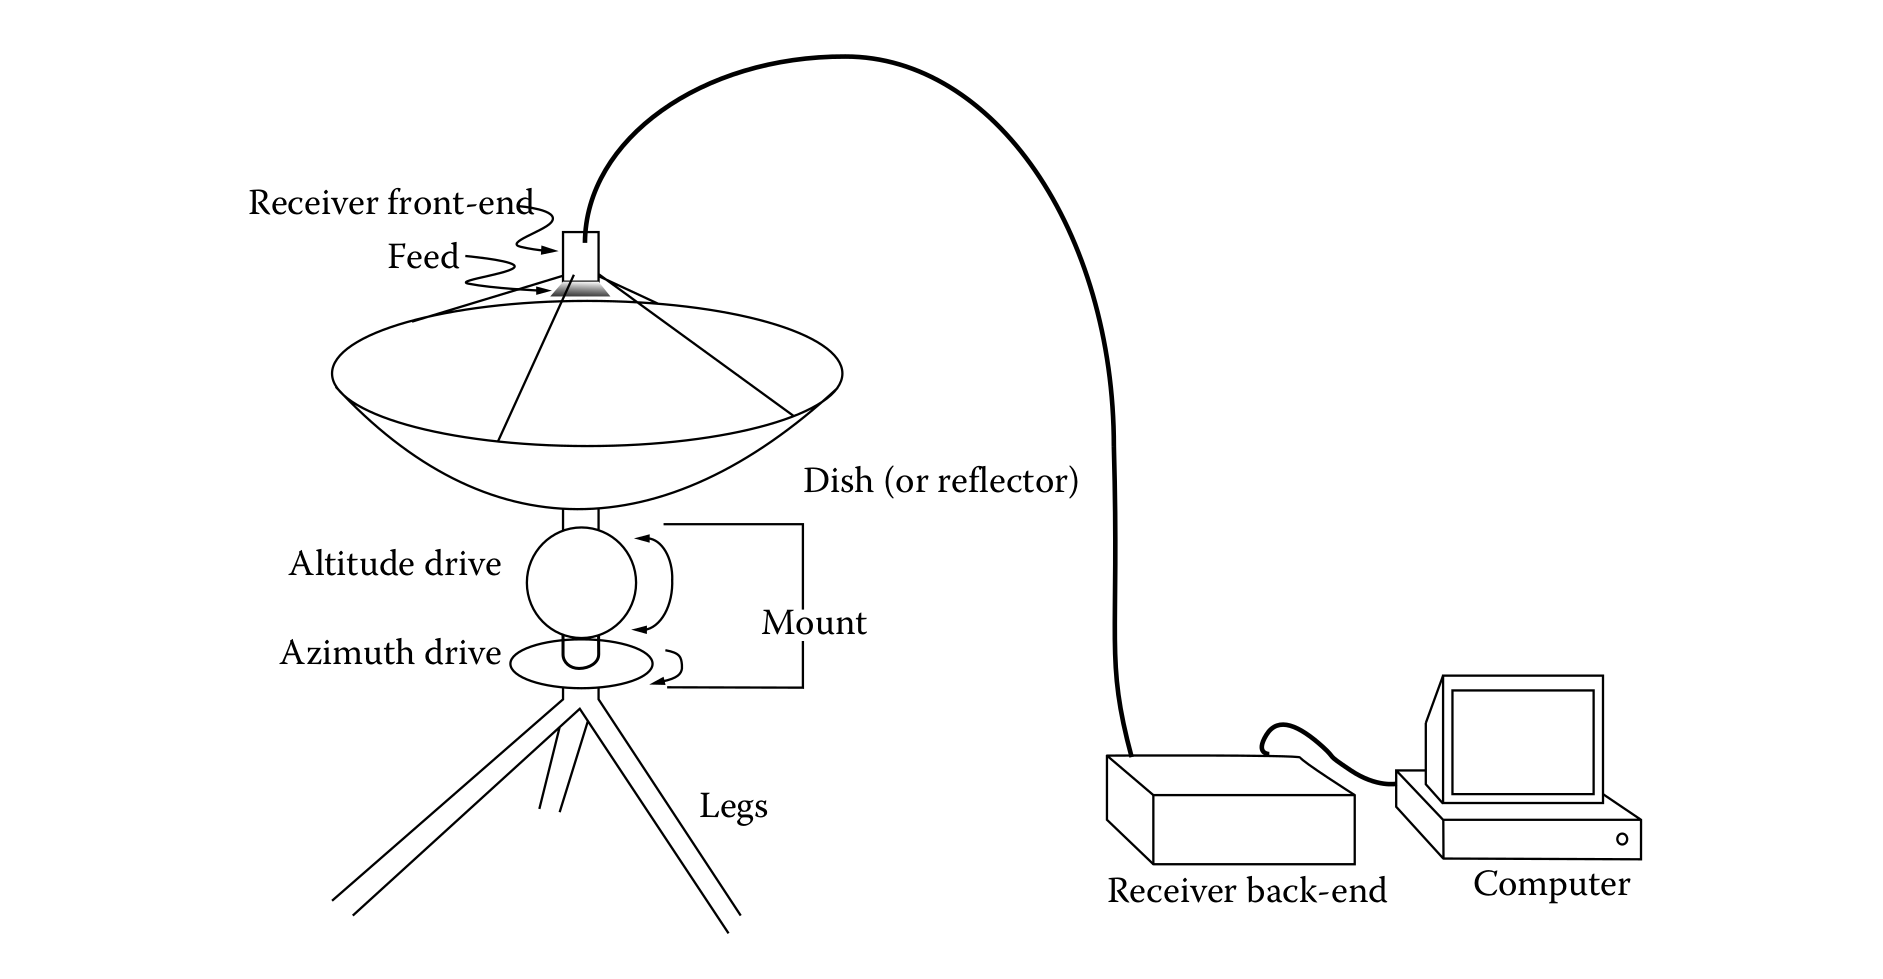
\includegraphics[width=0.5\textwidth]{Images/radio_telescope.png}
    \caption{A schematic diagram of a radio telescope.}
    \label{fig:radio_telescope}
\end{figure}

\subsection{Parabolic Reflector}
Most radio telescopes use a parabolic reflector (dish) to collect and focus radio waves. Unlike visible-light telescopes, radio telescopes do not use lenses. The radiation can be detected at the focal point (prime focus) or behind the dish (Cassegrain focus).

\begin{enumerate}
    \item The sensitivity of the telescope depends on the collecting area, proportional to the square of the reflector's diameter.
    \item Radio dishes do not need highly polished surfaces. Successful reflection occurs when surface irregularities are much smaller than the wavelength, \(\delta z < \frac{\lambda}{20}\). For longer wavelengths, the surface can be a mesh.
    \item The resolution of a radio telescope is determined by diffraction, improving with larger reflectors.
\end{enumerate}

\subsection{Mount}
The mount holds and moves the dish, allowing rotation around two axes. Modern radio telescopes use altitude-azimuth (Alt-Az) mounts, while older visible-wavelength telescopes often use equatorial mounts.

\subsection{Feeds, Receivers, and Computer}
The dish focuses radio waves to feeds that convert them into transmission lines, sending signals to receivers. The receiver front-end amplifies and processes the signal, which is then transmitted to the observatory's control room for further processing by the back-end and storage on a computer.

Each feed-receiver assembly acts like a pixel. Radio telescopes typically have fewer feed-receiver assemblies compared to the megapixel arrays in visible-wavelength telescopes due to the larger size and cost. Large telescopes like Arecibo and Green Bank can have 7 to 13 assemblies, while smaller ones like Haystack SRT have only one. At millimeter wavelengths, arrays with thousands of bolometer detectors exist.

Radio observations often yield fewer data points compared to visible-wavelength observations, but aperture synthesis (combining signals from multiple telescopes) can produce detailed images.

\clearpage

\section{Radio Maps}

Displaying the structure of a source at radio wavelengths requires choosing the best way to present two-dimensional data. There are three common approaches:

\subsection{Contour Maps}

The simplest way is using a contour map, where contours are lines of constant intensity, similar to a topographical map indicating lines of constant elevation. Closely spaced contours indicate regions where the intensity changes rapidly. An example of a contour map is shown in Figure~\ref{fig:contour_map}.

\begin{figure}[H]
    \centering
    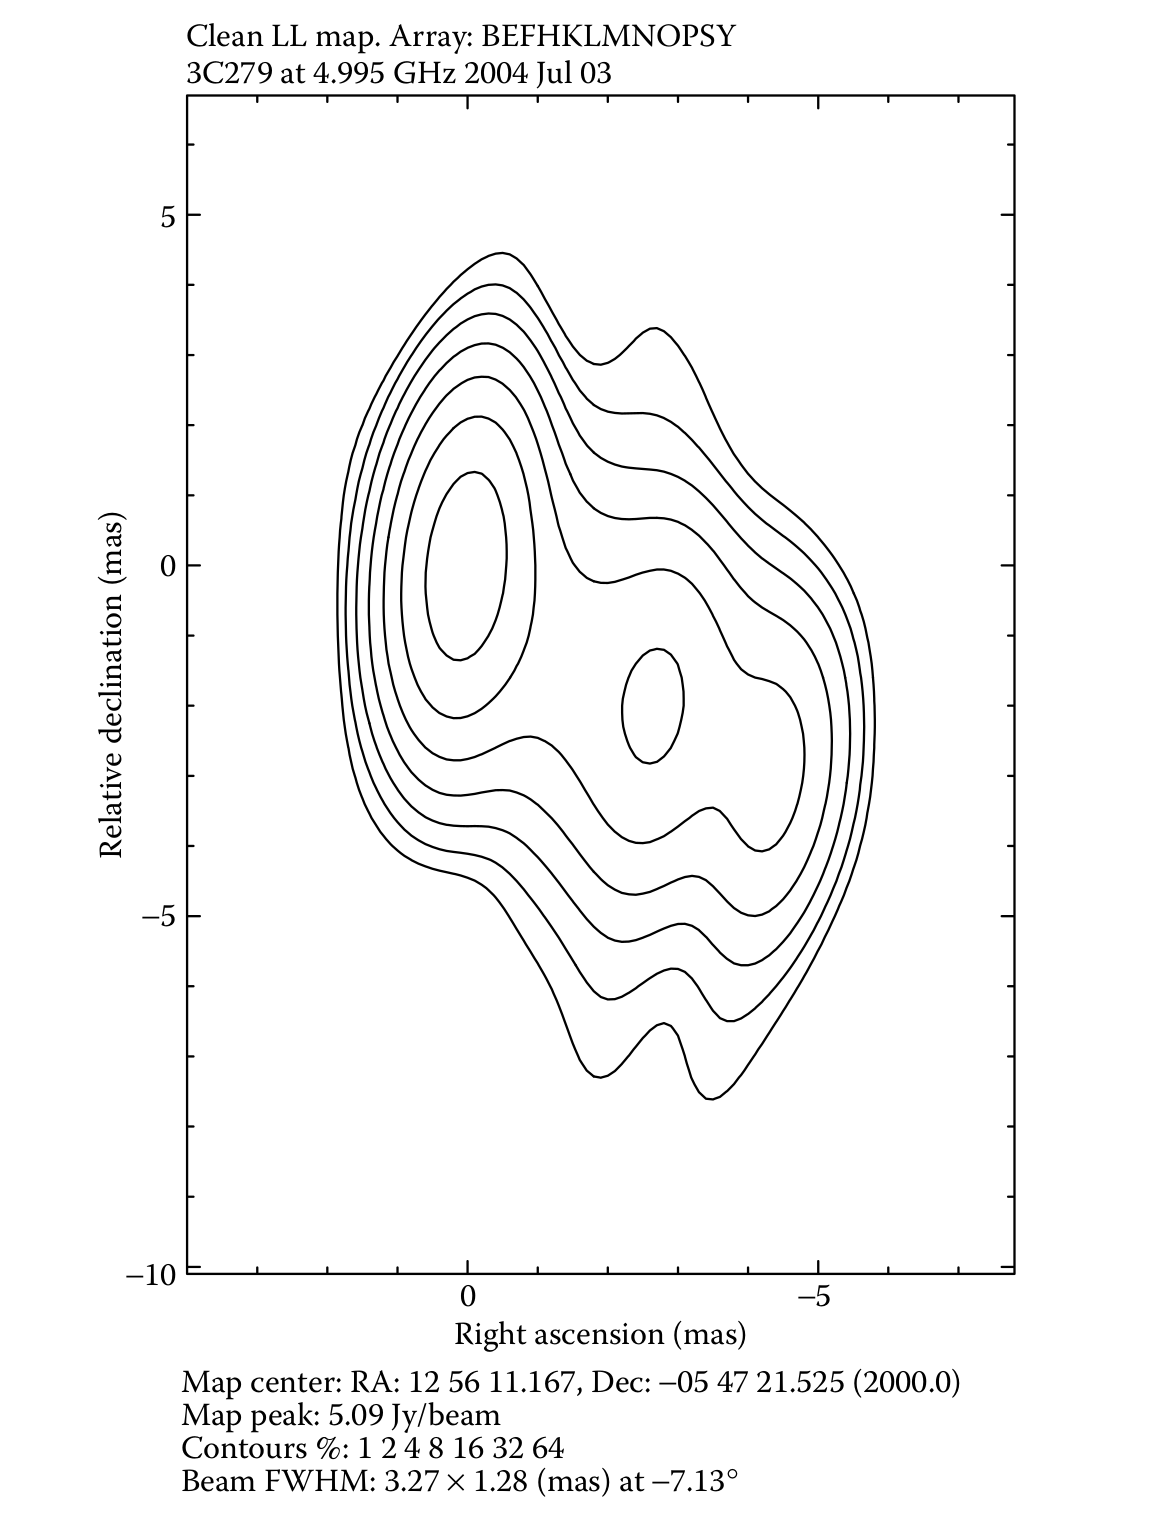
\includegraphics[width=0.7\textwidth]{Images/contour_map.png}
    \caption{An example of a contour map.}
    \label{fig:contour_map}
\end{figure}

\subsection{Gray Scale Maps}

A gray scale map directly indicates brightness variations with shades of gray, where black is the most intense and white the least. Although gray scale maps are more intuitive, they often do not reveal details as well as contour maps. Therefore, contour maps are preferred for detailed analysis. Overlaid gray scale and contour maps, as shown in Figure~\ref{fig:gray_scale_contour_overlay}, are common and visually pleasing.

\begin{figure}[H]
    \centering
    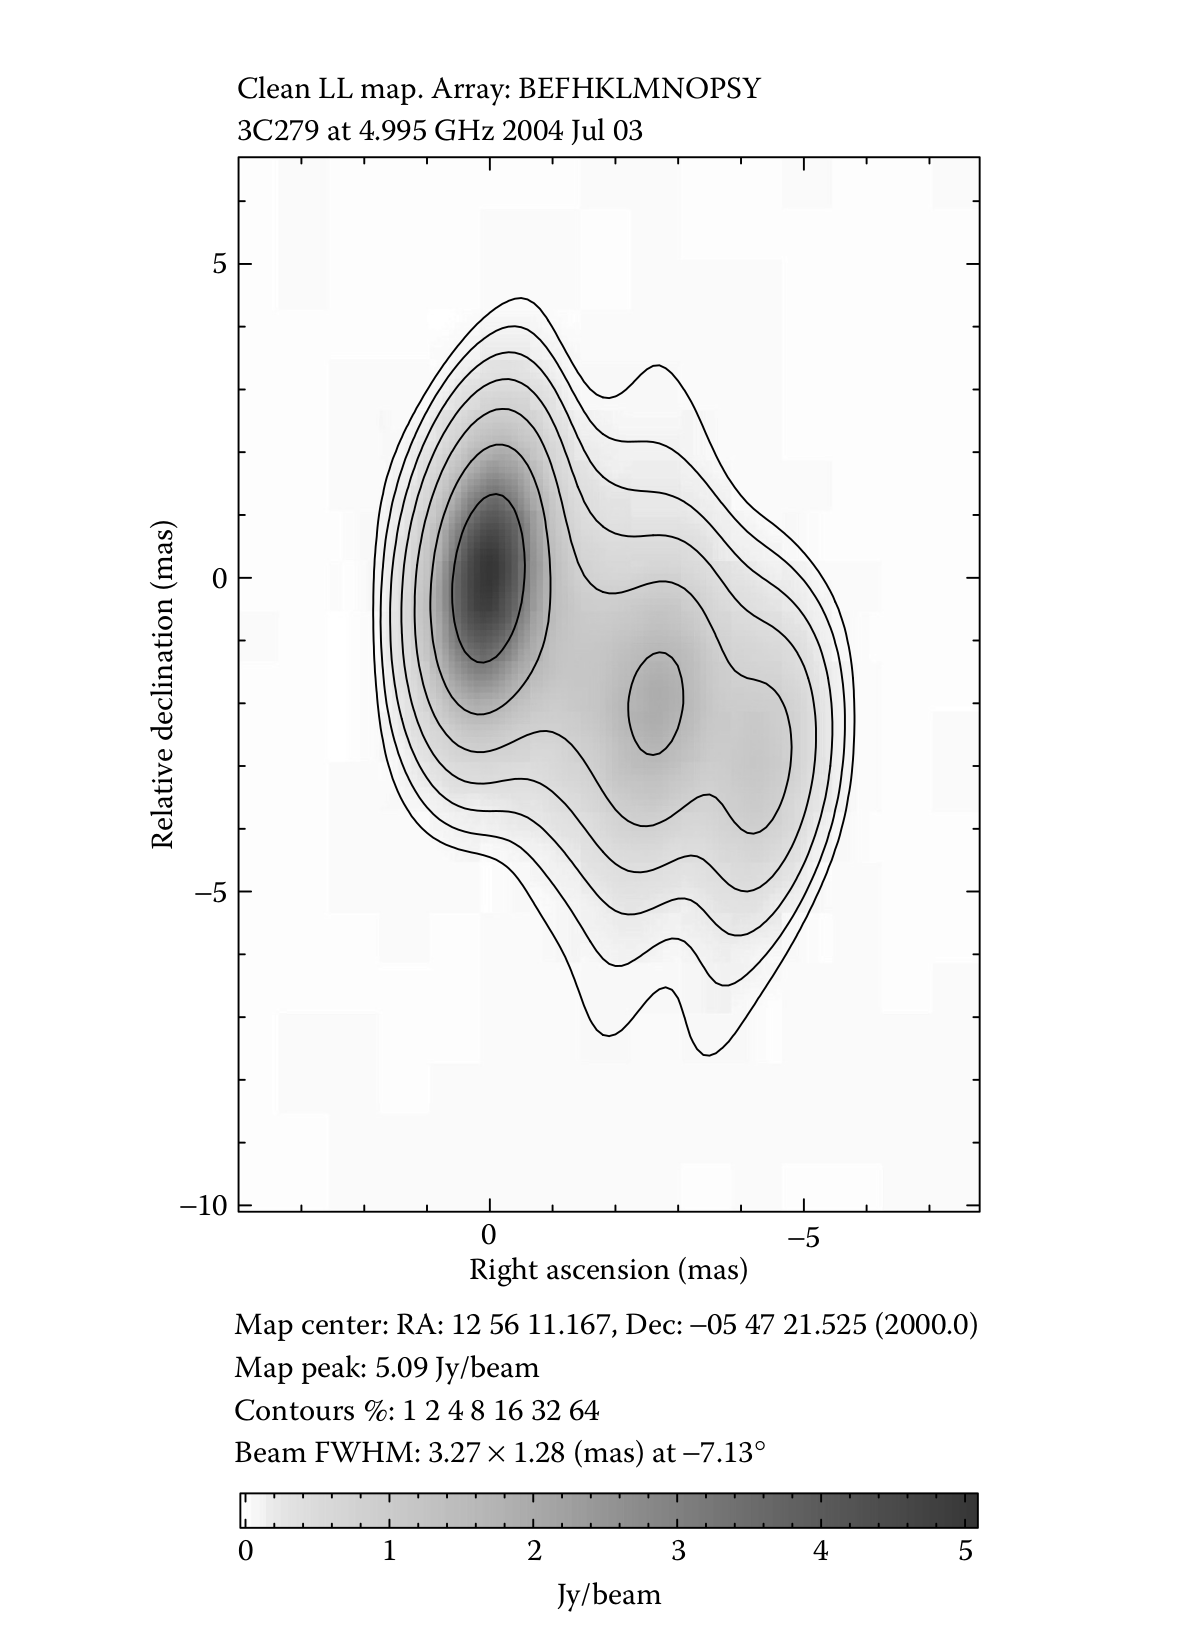
\includegraphics[width=0.7\textwidth]{Images/gray_scale_contour_overlay.png}
    \caption{An example of an overlaid gray scale and contour map.}
    \label{fig:gray_scale_contour_overlay}
\end{figure}

\subsection{False Color Maps}

False color maps use colors to indicate different levels of brightness rather than wavelengths. These images often include a color-wedge to show the relationship between color and brightness, facilitating analysis. An example of a false color map is shown in Figure~\ref{fig:false_color_map}.

\begin{figure}[H]
    \centering
    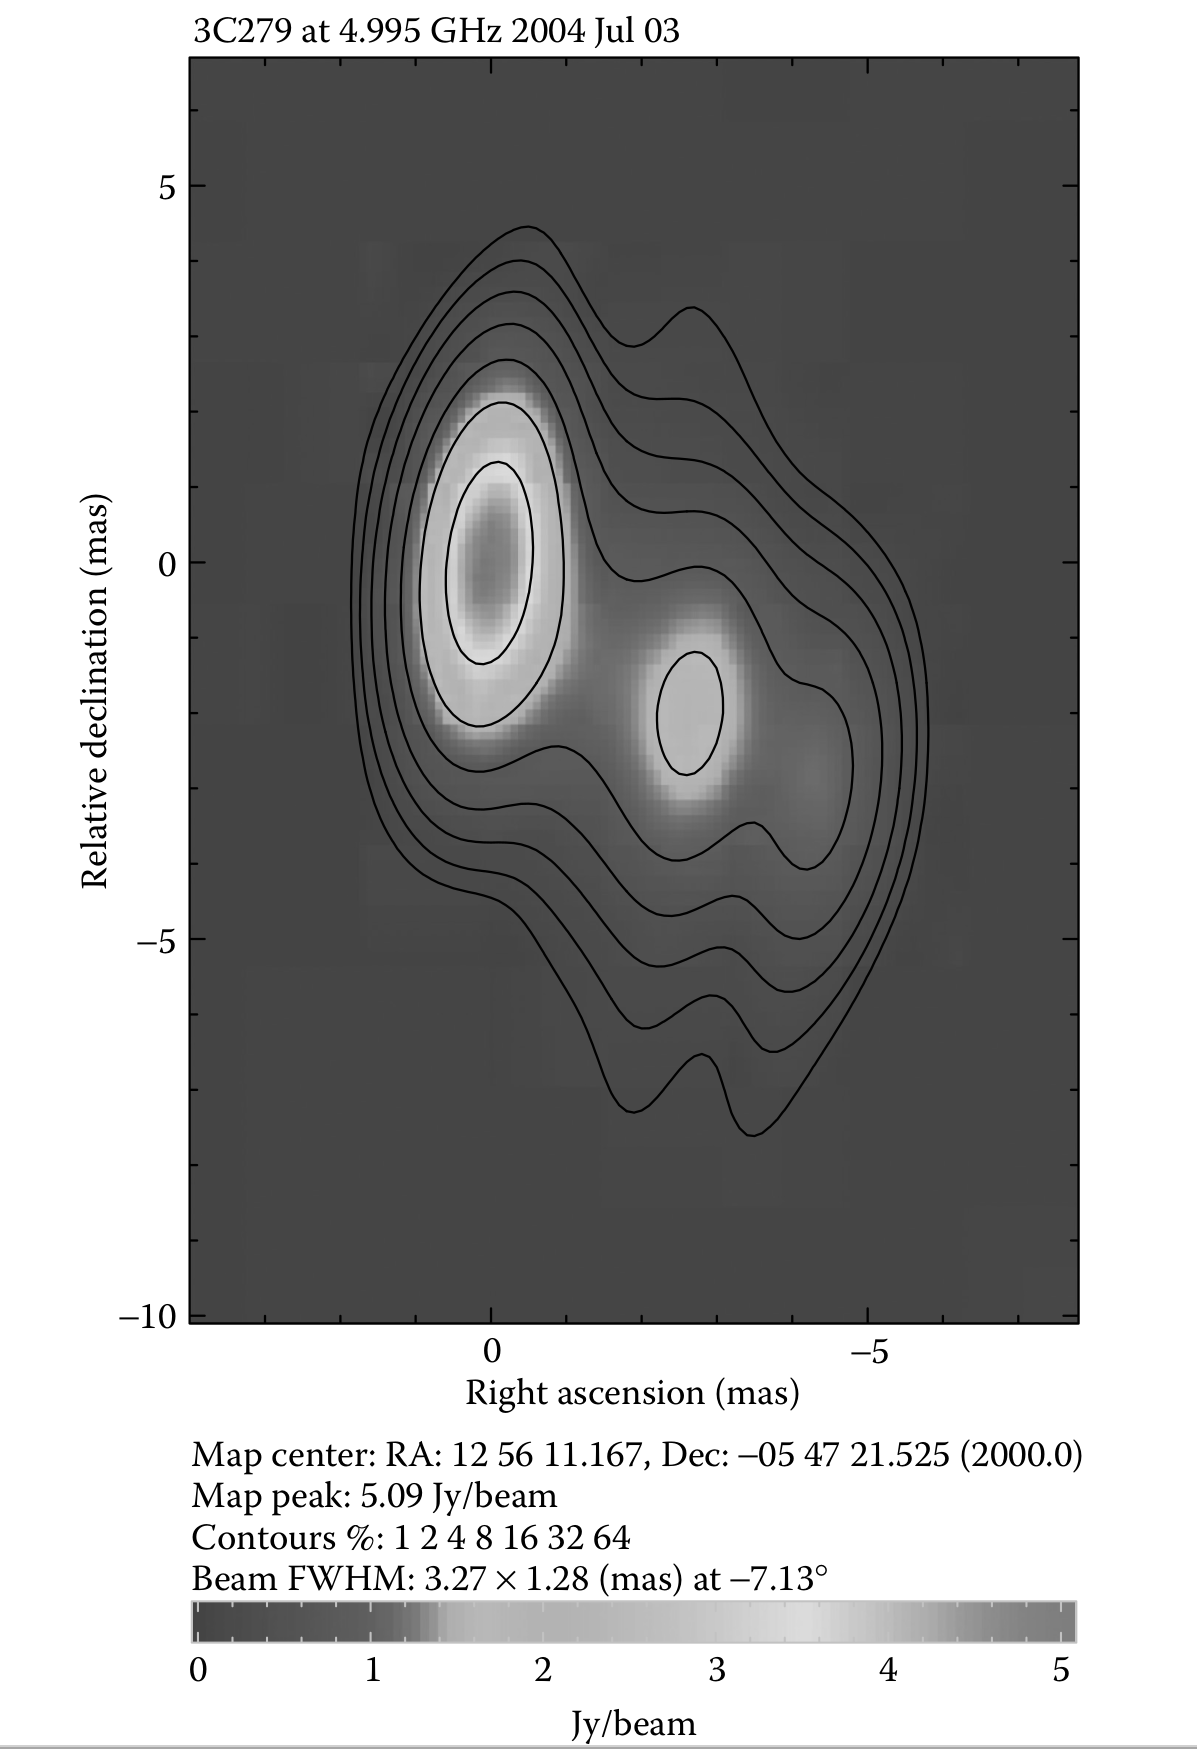
\includegraphics[width=0.6\textwidth]{Images/false_colour_map.png}
    \caption{An example of a false color map.}
    \label{fig:false_color_map}
\end{figure}

\subsection{Multicolor Images}

Radio astronomers sometimes create multicolor images similar to visible light astronomers. By observing several different radio wavelengths, images can be overlaid, assigning red to the longest wavelength, green to intermediate wavelengths, and blue to the shortest wavelength.


\clearpage

\section{Galaxy FITS Data in Multiple Wavelengths}

We will choose 3 Galaxies - Sunflower, Tadpole and Whirlpool Galaxy, and use the CIRADA image cutout web service to display their FITS data in multiple wavelengths. This service enables us to obtain optical, infrared, and radio images of all three galaxies.

Different wavelengths reveal different aspects of the galaxies. Optical images show the distribution of stars, while infrared images reveal the distribution of dust and gas. Radio images show the distribution of cold gas and synchrotron radiation from cosmic rays.

\subsection{Sunflower Galaxy}

\begin{figure}[H]
    \centering
    \includegraphics[width=\textwidth]{Images/sunflower.png}
    \caption{Sunflower Galaxy in multiple wavelengths.}
    \label{fig:sunflower}
\end{figure}

\subsection{Tadpole Galaxy}
    
\begin{figure}[H]
    \centering
    \includegraphics[width=\textwidth]{Images/tadpole.png}
    \caption{Tadpole Galaxy in multiple wavelengths.}
    \label{fig:tadpole}
\end{figure}

\subsection{Whirlpool Galaxy}

\begin{figure}[H]
    \centering
    \includegraphics[width=\textwidth]{Images/whirlpool.png}
    \caption{Whirlpool Galaxy in multiple wavelengths.}
    \label{fig:whirlpool}
\end{figure}

\clearpage

\section{Jet Afterglow Lightcurve of GW170817}

GW170817 was a merger of two neutron stars that was accompanied by both gravitational waves and electromagnetic radiation. We used the data for the non-thermal emission from this source that spans across all frequency bands following a single spectral index of $F_{\nu} \propto {\nu}^{-0.584}$ . The quantity F is the flux density, which measures the amount of energy incident on the detector per unit area of the detector, an indicator of the brightness of the source. A lightcurve is this flux density represented as a function of time. 

We plotted the lightcurve choosing all the VLA 3 GHz data points.

\begin{figure}[H]
    \centering
    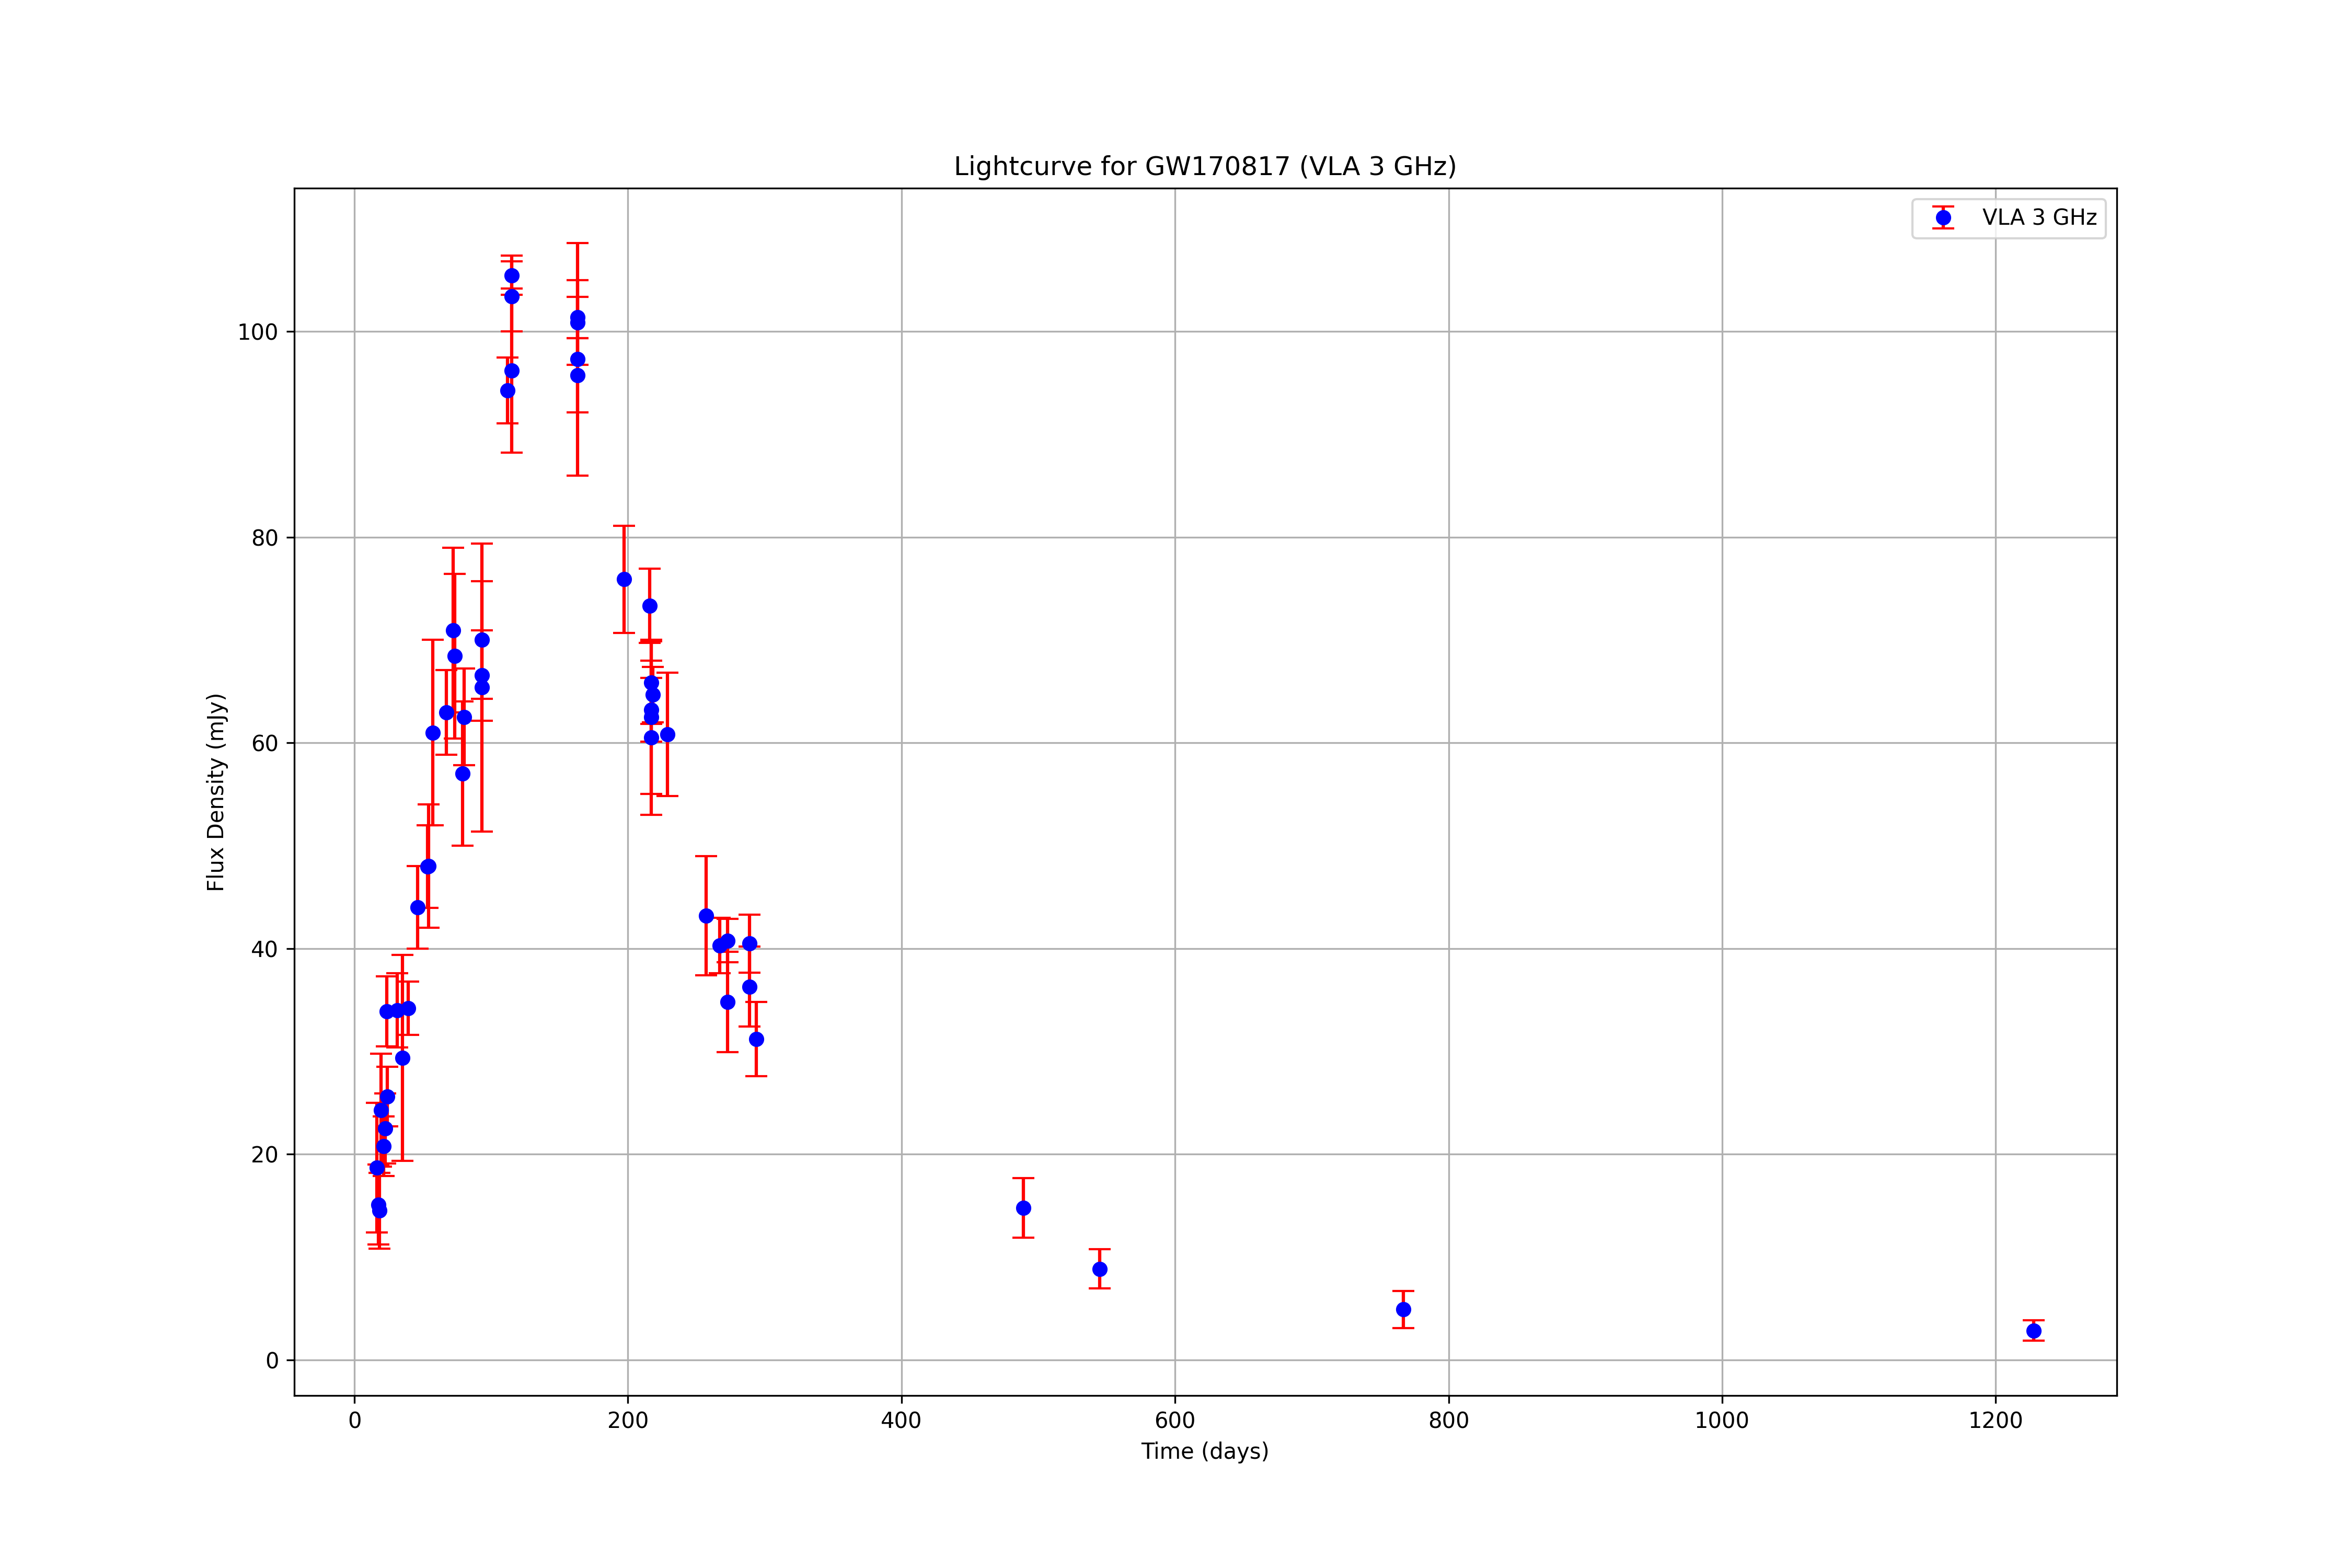
\includegraphics[width=0.6\textwidth]{Images/vla_lightcurve.png}
    \caption{Flux Density vs Time at 3GHz frequency measured by VLA telescope.}
    \label{fig:vla_lightcurve}
\end{figure}

\vspace{10mm}

We also plotted the lightcurve choosing all the Chandra 3 GHz data points.

\begin{figure}[H]
    \centering
    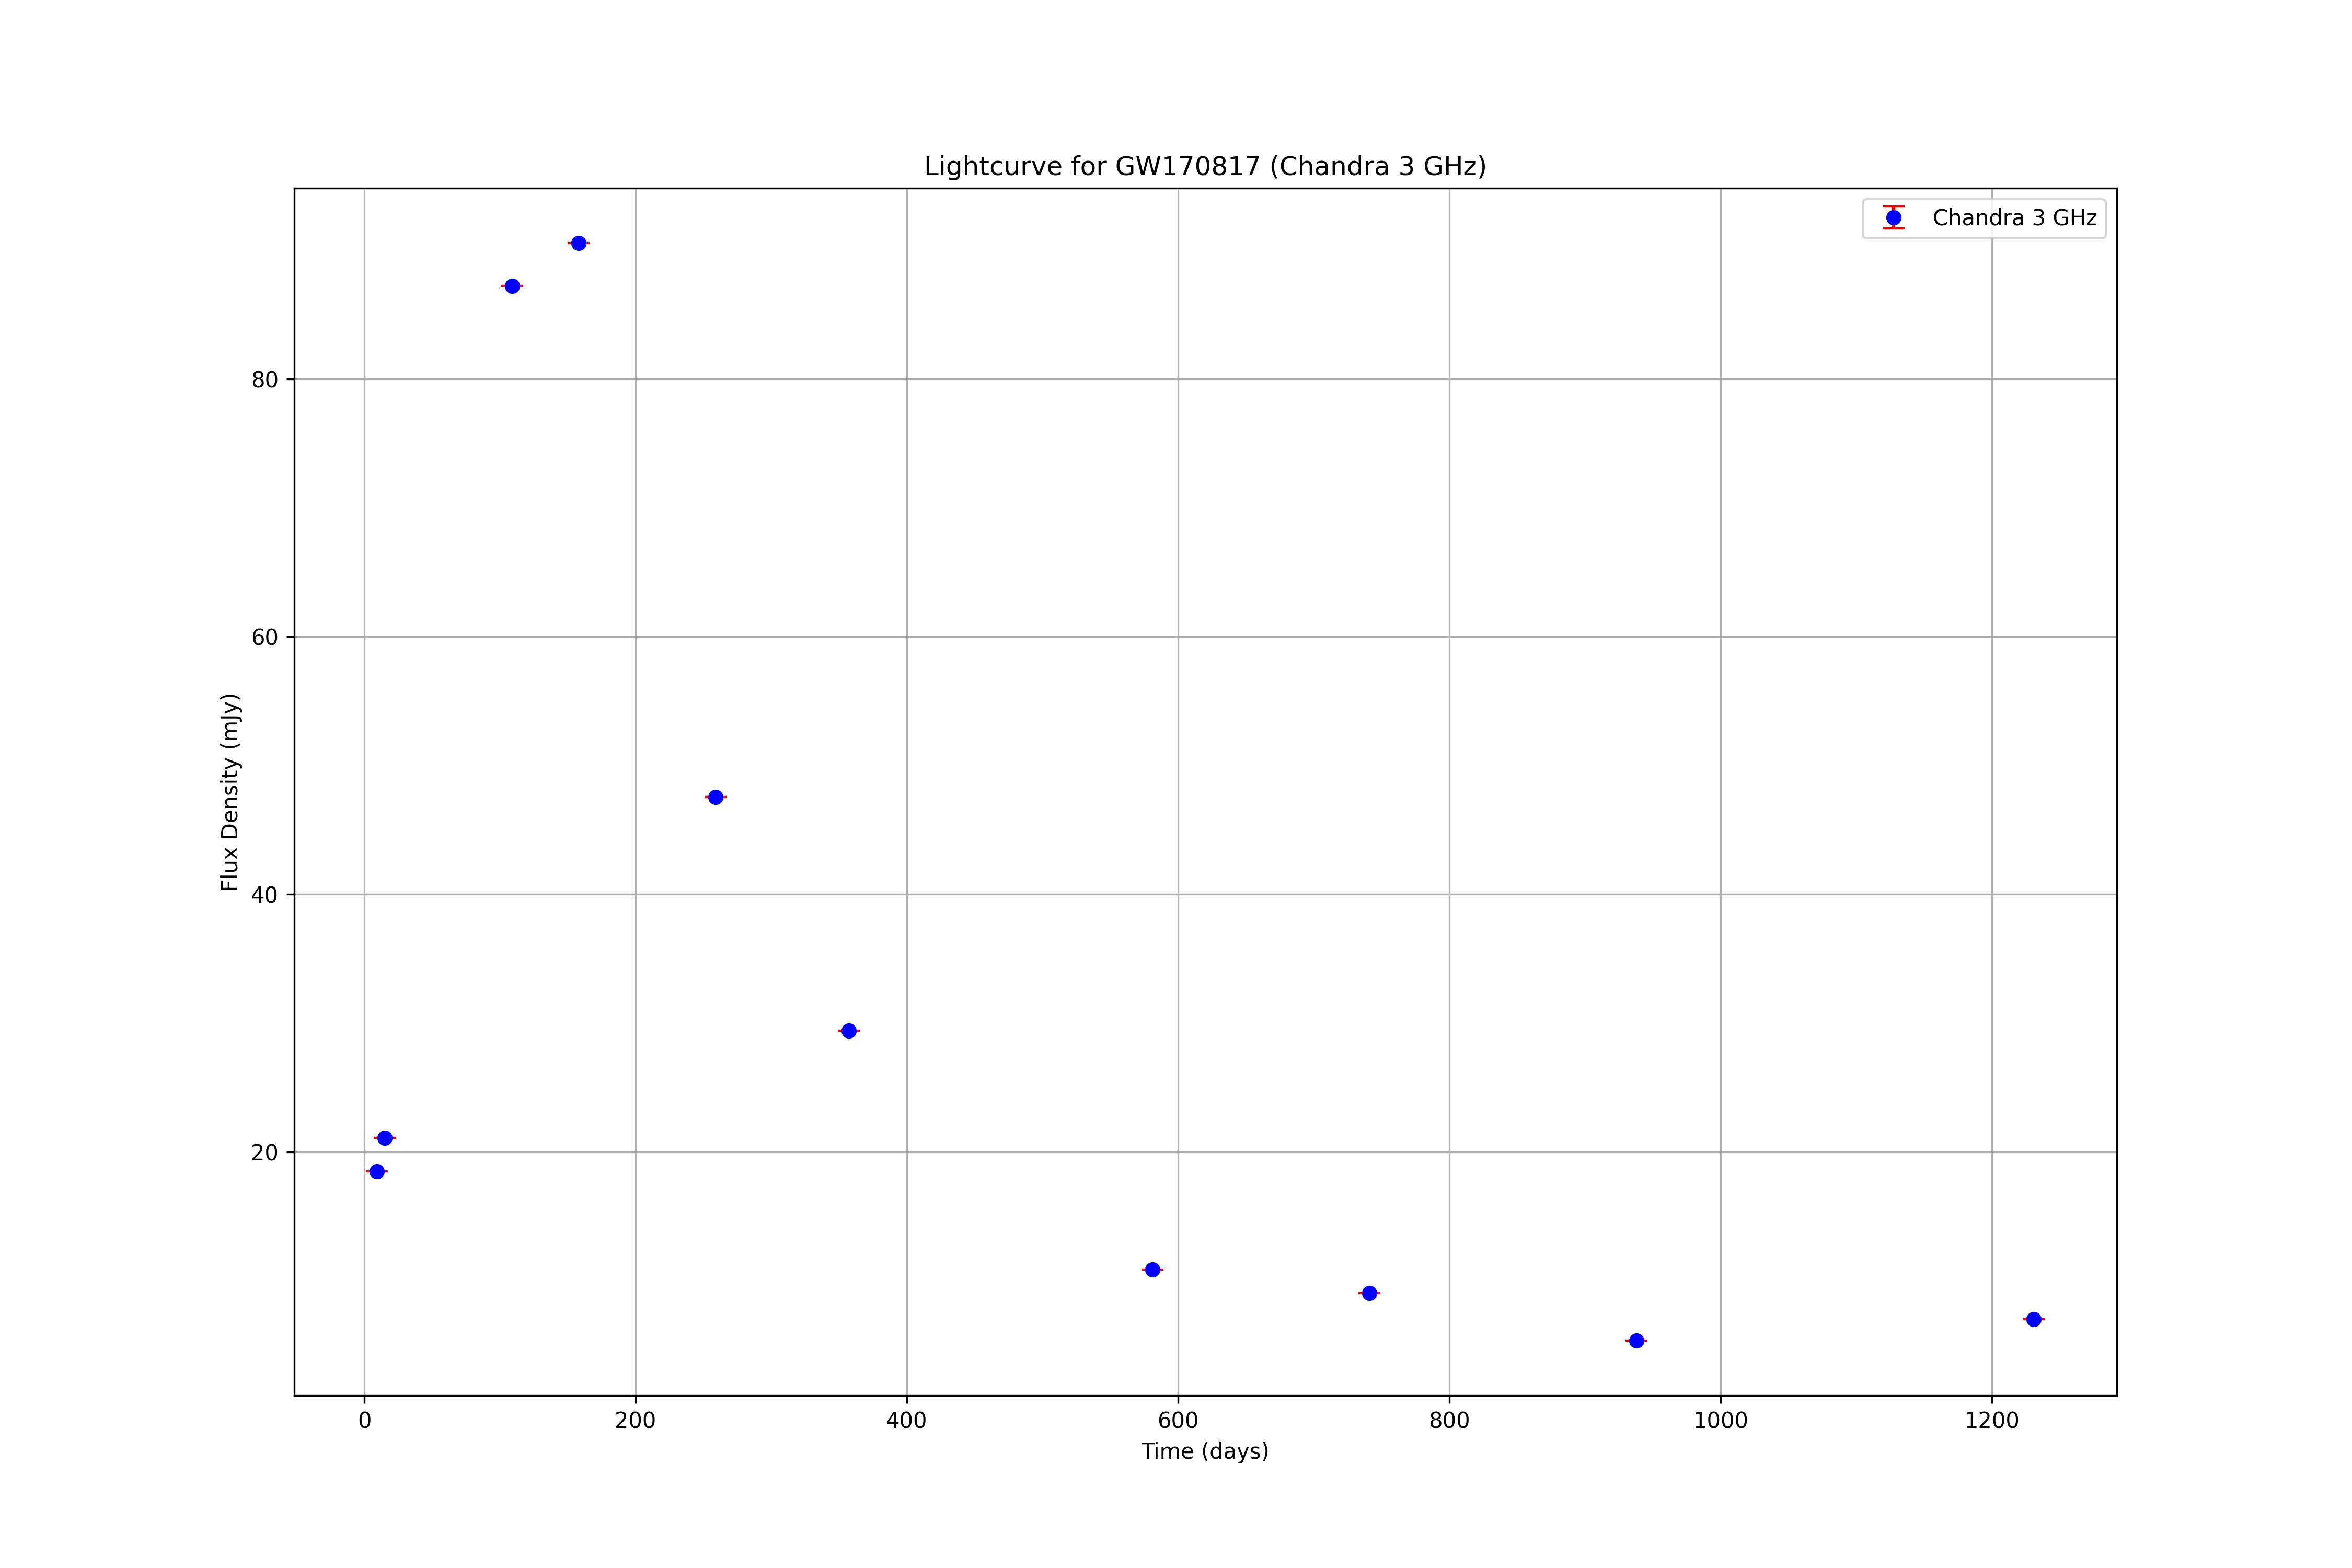
\includegraphics[width=0.6\textwidth]{Images/chandra_lightcurve.png}
    \caption{Flux Density vs Time at 3GHz frequency measured by Chandra telescope.}
    \label{fig:chandra_lightcurve}
\end{figure}

